{
  \definecolor{trans-fb}{RGB}{215, 48, 31}
  \definecolor{trans-lb}{RGB}{252, 141, 89}
  \definecolor{trans-exn}{RGB}{147, 204, 0}
  \definecolor{erasure}{RGB}{119, 133, 254}

  \newcommand\config[1]{\begin{minipage}{0.09\textwidth}\centering\includegraphics[width=\linewidth]{Images/#1}\end{minipage}}
  \newcommand\runtimeError{\begin{minipage}{0.03\textwidth}\centering
\includegraphics[width=\linewidth]{Images/runtime-error}\end{minipage}}
  \newcommand\checkFailure{\begin{minipage}{0.03\textwidth}\centering\includegraphics[width=\linewidth]{Images/check-failure-plain}\end{minipage}}
  \newcommand\blameFinger{\begin{minipage}{0.02\textwidth}\centering\vspace{0.25em}\includegraphics[width=\linewidth]{Images/finger}\end{minipage}}
  \newcommand\typeError{\scalebox{1.5}{$\tau_{\hspace{-0.1em}\times}$}}
  \newcommand\success{\textcolor{black!30!green}{\LARGE \checkmark}}
  \newcommand\fail{\textcolor{red}{\LARGE \sffamily x}}
  \footnotesize
\centering
\begin{tabular}{l|ccl|ccl|cc|c}
\multicolumn{3}{c}{\begin{minipage}{0.25\textwidth}\centering\includegraphics[width=\linewidth]{Images/take5-module-graph}\end{minipage}} &
\multicolumn{7}{c}{\begin{minipage}{0.69\textwidth}\centering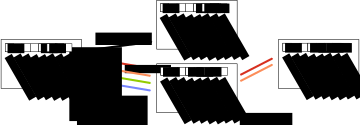
\includegraphics[width=\linewidth]{Images/trails-example}\end{minipage}} \\
\multicolumn{3}{c}{\begin{minipage}{0.25\textwidth}\centering the dependency graph\end{minipage}} &
\multicolumn{7}{c}{\begin{minipage}{0.69\textwidth}\centering the paths taken by each mode through the configuration lattice\end{minipage}} \\
\end{tabular}
\vspace{1em}

\begin{tabular}{l|ccl|ccl|cc|c}
 & \textbf{Root} &  &  & \textbf{Step 1} &  &  & \textbf{Step 2} &  & \textbf{Success?}\\
\textbf{Mode} & config & result & stack & config & result & stack & config & result & \\
\hline
Natural & \config{10001100} & \blameFinger & \texttt{main} & \config{10001110} & \typeError &  &  &  & \success\\
-blame &  & \texttt{player} & \texttt{main} &  &  &  &  &  & \\
\hline
\textcolor{trans-fb}{Transient} & \config{10001100} & \runtimeError & \texttt{dealer} & \config{10011100} & \blameFinger & \texttt{dealer} & \config{10011110} & \typeError & \success\\
\textcolor{trans-fb}{-first-blame} &  &  & \texttt{dealer} &  & \texttt{player} &  &  &  & \\
\emph{and} &  &  & \texttt{dealer} &  & \texttt{dealer} &  &  &  & \\
\textcolor{trans-lb}{-last-blame} &  &  & \texttt{main} &  &  &  &  &  & \\
\hline
\textcolor{erasure}{Erasure} & \config{10001100} & \runtimeError & \texttt{dealer} & \config{10011100} & \runtimeError & \texttt{dealer} &  &  & \fail\\
 &  &  & \texttt{dealer} &  &  & \texttt{dealer} &  &  & \\
 &  &  & \texttt{dealer} &  &  & \texttt{dealer} &  &  & \\
 &  &  & \texttt{main} &  &  & \texttt{main} &  &  & \\
\hline
\textcolor{gray}{Natural} & \config{10001100} & \checkFailure & \texttt{main} &  &  &  &  &  & \fail\\
\textcolor{gray}{-exceptions} &  &  & \texttt{main} &  &  &  &  &  & \\
\hline
\textcolor{trans-exn}{Transient} & \config{10001100} & \runtimeError & \texttt{dealer} & \config{10011100} & \checkFailure & \texttt{dealer} &  &  & \fail\\
\textcolor{trans-exn}{-exceptions} &  &  & \texttt{dealer} &  &  &  &  &  & \\
 &  &  & \texttt{dealer} &  &  &  &  &  & \\
 &  &  & \texttt{main} &  &  &  &  &  & \\
\end{tabular}

\begin{minipage}{0.95\textwidth}
\vspace{0.5em}
\centerline{\it Legend}

\noindent{\it config} \hspace{0.5em} Each box corresponds to a module and indicates (with x) if it is typed. 
The mutated module is gray.

\medskip

\noindent{\it result}\\
\begin{center}
\vspace{-2.5em}
\begin{tabular}{c@{\quad}l}
symbol        & denotation \\ \hline 
\blameFinger  & the configuration signals a dynamic type check failure, blaming the module(s) below \\
\typeError    & the configuration does not type check\\
\runtimeError & the configuration fails a check by the runtime system\\
\checkFailure & the configuration signals a dynamic type check failure for which blame is ignored\\
\end{tabular}
\end{center}

\end{minipage}}

